\begin{problem}
    \p
جمله عمومی دنباله زیر را به دست آورید.
	\p
	\begin{center}
		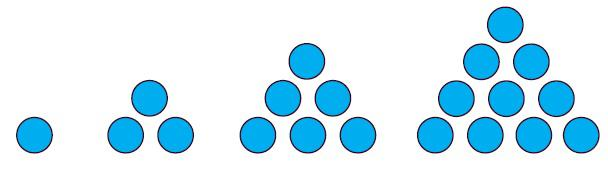
\includegraphics[scale=0.3]{./1.jpg}
	\end{center}
    \problemsolution{
        \p
       هر مثلث نسبت به مثلث قبلی یک ردیف بیشتر دارد یعنی: 
    		$$a_1 = 1$$
    		$$a_2 = a_1 + 2$$
    		$$a_3 = a_2 + 3$$
    		$$\vdots$$
    		$$\Downarrow$$
    		$$a_n = a_{n-1} + n$$
            $$a_1 + a_2 + ... + a_n = a_1 + a_2 + ... + a_{n-1} + 1 + 2 + ... + n$$
            $$a_n = 1 + 2 + 3 + ... + n = \frac{n(n+1)}{2}$$
        }
\end{problem}